\documentclass[a4paper,11pt]{article}

% Packages
\usepackage[utf8]{inputenc}
\usepackage{geometry}
\usepackage{amsmath, amssymb}
\usepackage{graphicx}
\usepackage[colorinlistoftodos]{todonotes}

% Page setup
\geometry{margin=2.5cm}

% Title info
\title{Assignment 3: Machine Learning for Time Series}
\author{Frederik Appel Vardinghus-Nielsen}
\date{\today}

\begin{document}

\maketitle
\listoftodos

\section{FD001: Single Condition, Single Fault Mode}

\subsection{Problem understanding}
The RUL task is a regression problem since the target variable is a time period. The variable in this task is in a unit of cycles, which are strictly discrete, but there are no predefined classed and the range has no upper bound, so regression is more fitting.

One row in the dataset represents one cycle, the unit of time. Each row contains info on engine value, operation settings, time and sensor values.

RUL labels must be constructed from the given failure time in cycle number.
\begin{itemize}
\item The train series run until failure, so the labels will be the total number of cycles minus the current cycle number.
\item The test series do not run until failure but the number of cycles until failure when the series ends is given so the labels will be the length of the test series plus the RUL at the end of the series minus the current cycle number.
\end{itemize}

\subsection{Exploratory data analysis}

Figure~\ref{fig:lifetime_dist} shows the distribution of engine lifetimes in the FD001 training set.
The lifetimes range from roughly 130 to 360 cycles with most engines failing between 150 and 250 cycles.

\begin{figure}[h]
    \centering
    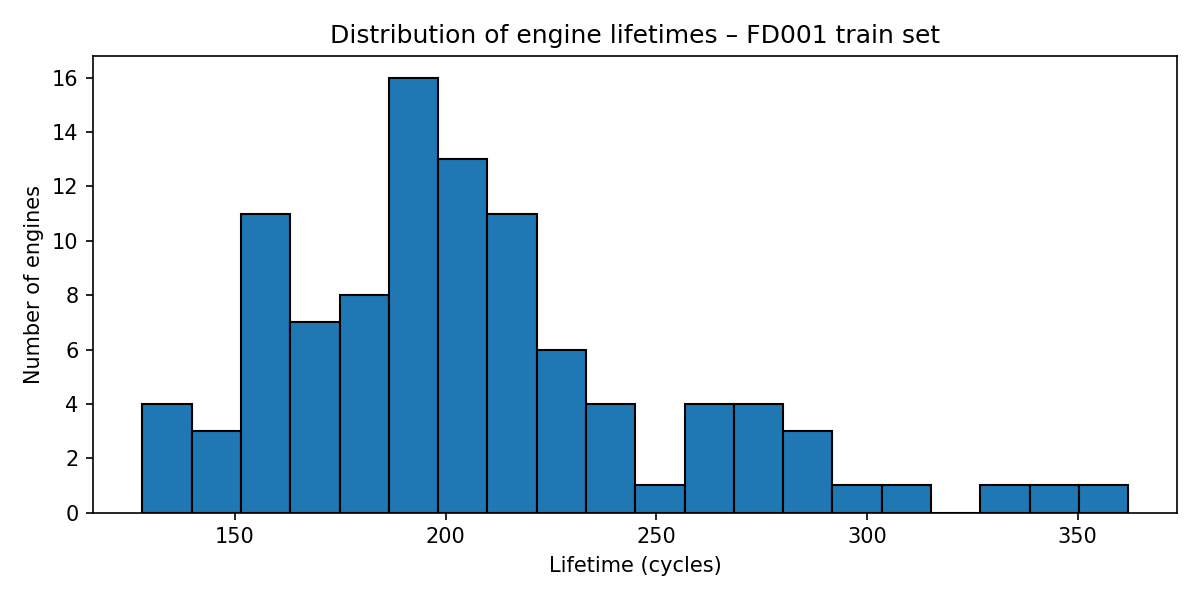
\includegraphics[width=0.7\textwidth]{../src/results/figures/lifetime_distribution.png}
    \caption{Distribution of engine lifetimes in the FD001 training set.}
    \label{fig:lifetime_dist}
\end{figure}

Figure~\ref{fig:sensor_traj} shows the raw sensor trajectories for a sample of engines.
Many sensors are constant (e.g.\ \texttt{sensor\_1}, \texttt{sensor\_5}) and carry no degradation signal, while others (e.g.\ \texttt{sensor\_2}, \texttt{sensor\_11}) show a clear monotonic trend over the engine lifetime.

\begin{figure}[h]
    \centering
    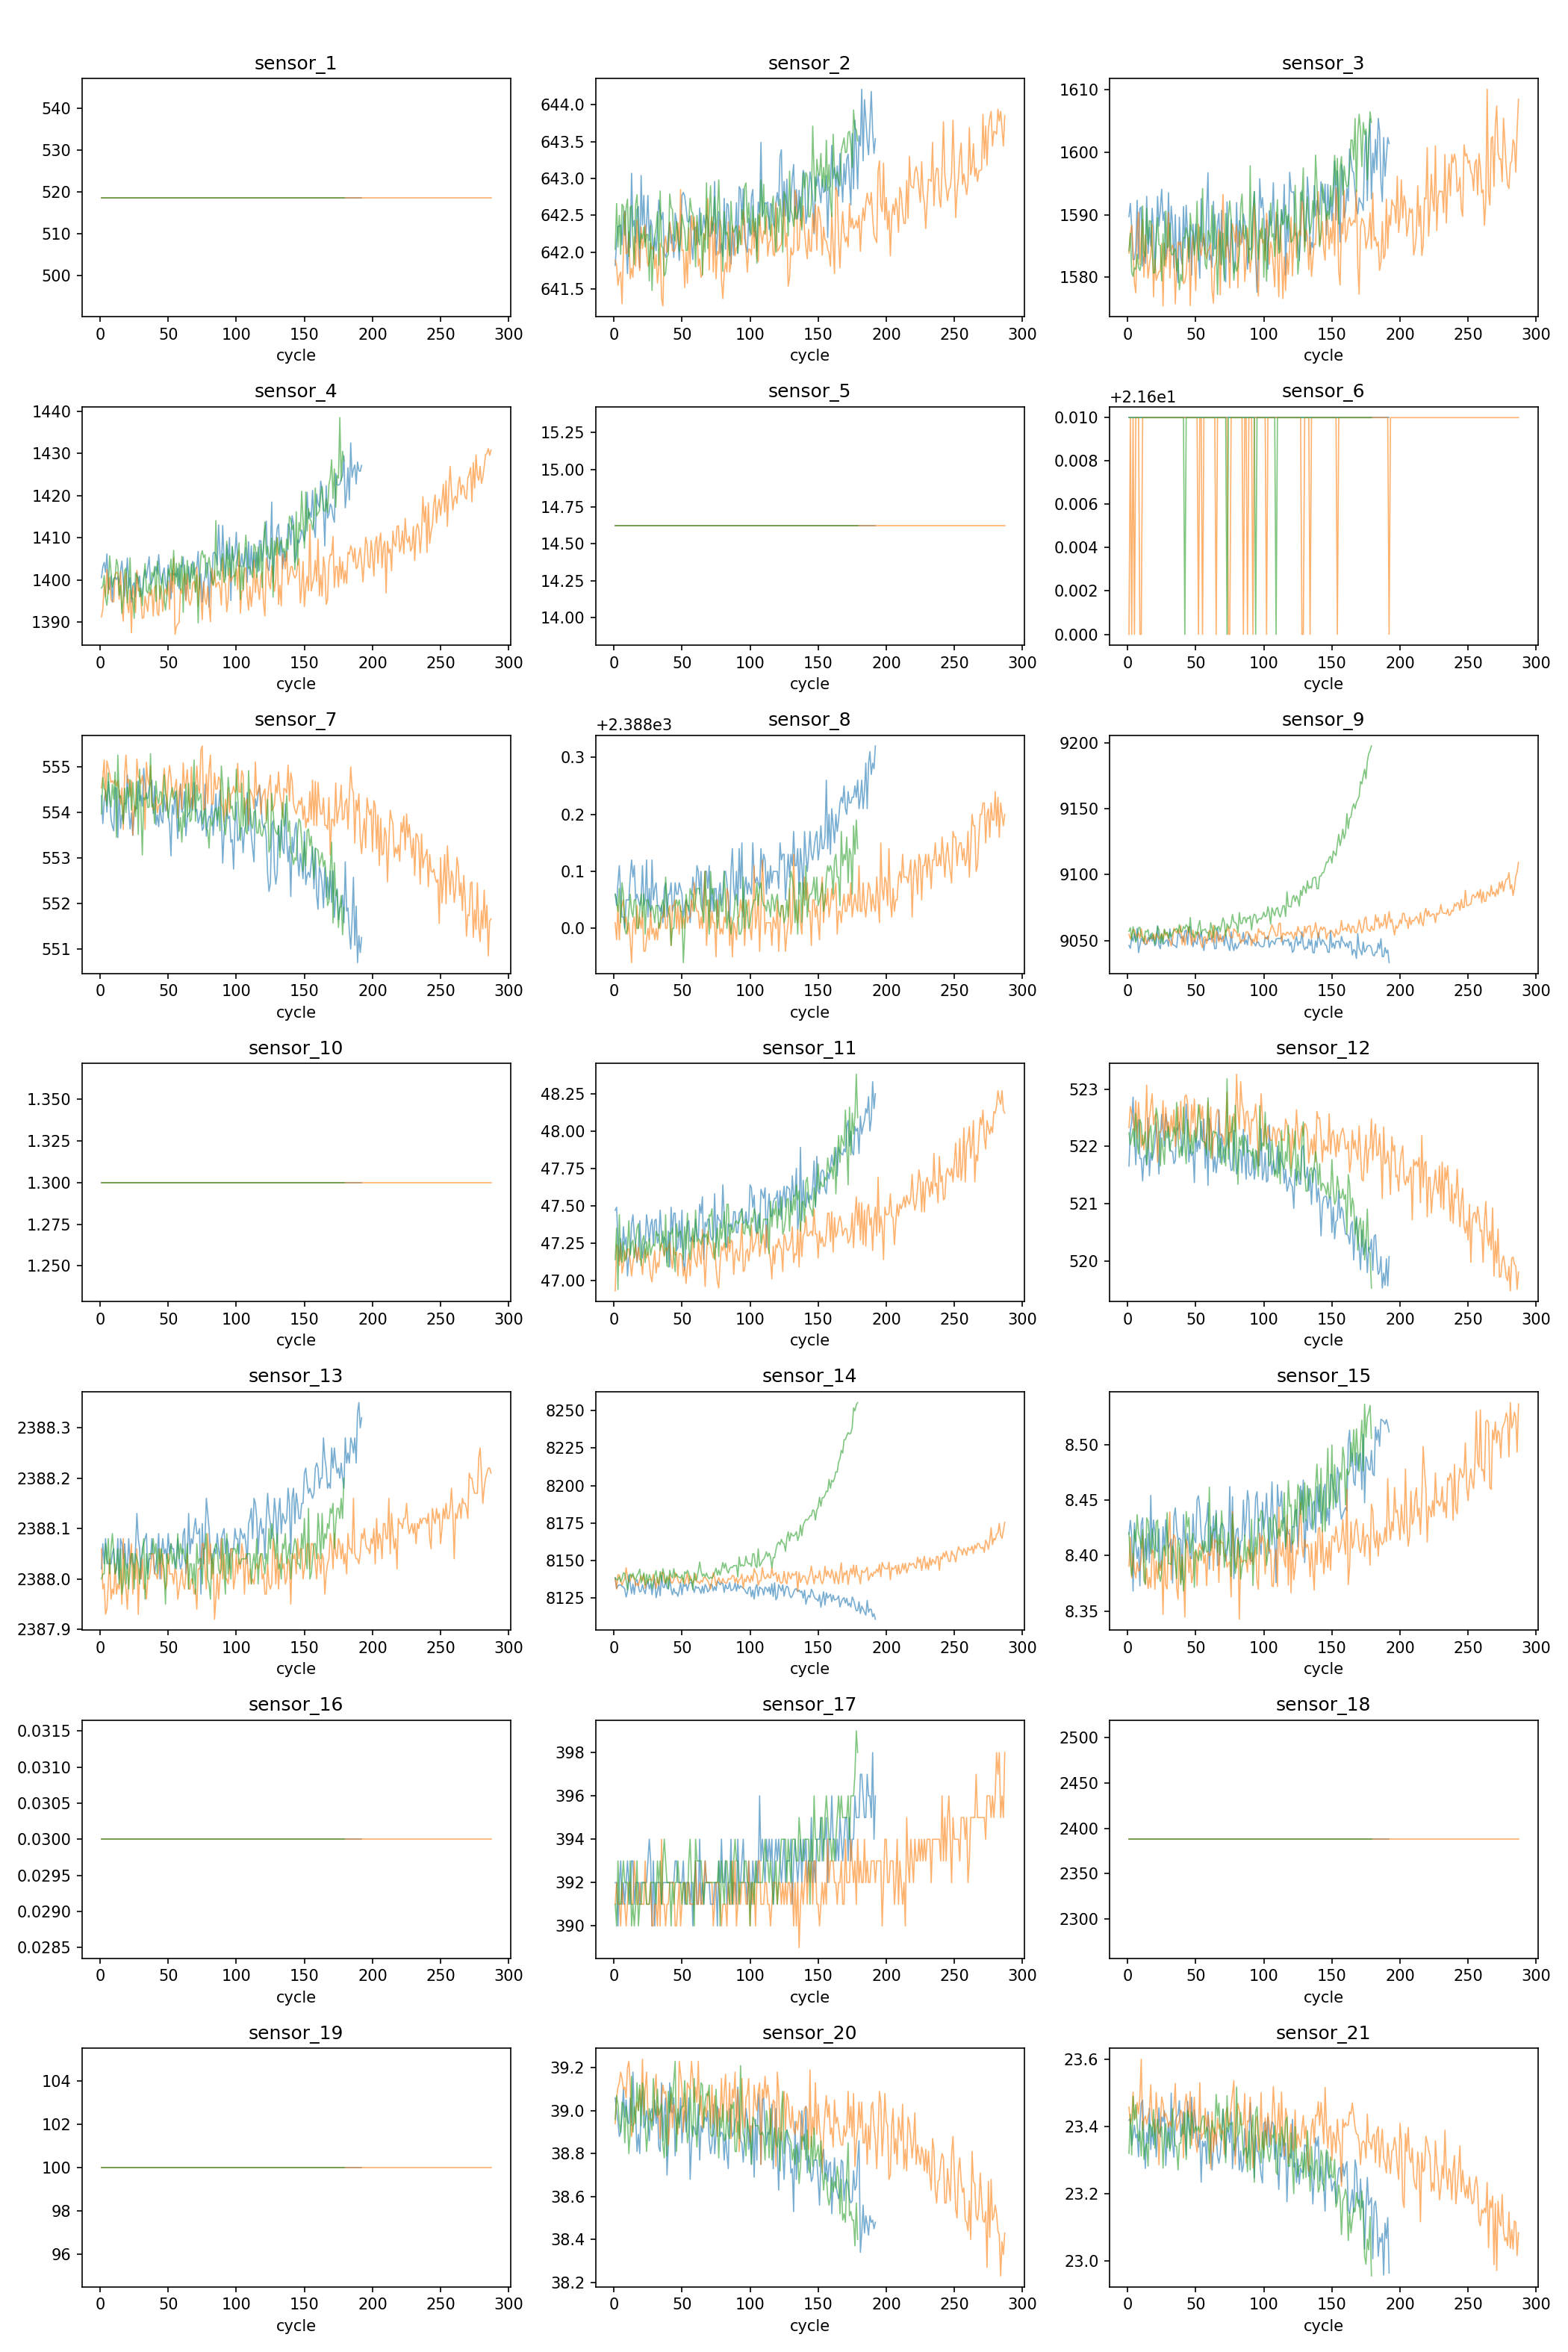
\includegraphics[width=0.6\textwidth]{../src/results/figures/sensor_trajectories.png}
    \caption{Per-sensor trajectories for a sample of engines in the FD001 training set.}
    \label{fig:sensor_traj}
\end{figure}

The sensor channels were chosen based upon their Spearman correlation with the cycle number. The Spearman correlation was calculated individually for each sensor for each engine and then aggregated across engines by mean. The sensor channels with mean Spearman correlation above 0.5 and standard deviation below 0.3 were selected. This resulted in 12 sensors: \texttt{sensor\_2}, \texttt{sensor\_3}, \texttt{sensor\_4}, \texttt{sensor\_7}, \texttt{sensor\_8}, \texttt{sensor\_11}, \texttt{sensor\_12}, \texttt{sensor\_13}, \texttt{sensor\_15}, \texttt{sensor\_17}, \texttt{sensor\_20}, and \texttt{sensor\_21}.

\subsection{Data preparation}
\begin{itemize}
\item \textbf{RUL label construction:} constructed as piecewise-linear with a cap of 125 cycles. RUL beyond 125 is not expected to show sensor values that are much different from other healthy data points, so capping prevents the model from attempting to learn less relevant patterns and focus of the part where health deterioration is more evident.
\item \textbf{Train/validation split:} A classic 80/20 split by engines for train/val is used.
\item \textbf{Normalization:} The sensor values are normalized by subtracting the mean and dividing by the standard deviation of each sensor channel across engines in the training set. This is classic Z-score normalization, which ensures that all sensor channels are on a comparable scale and prevents any single channel from dominating the learning process due to larger numeric values.
\item \textbf{Fixed random seed:} A fixed random seed (42) for the train/validation split is used to ensure reproducibility.
\end{itemize}
\subsection{Feature engineering -- raw fixed-window pipeline}
A window length $w=30$ is used. This is treated as a hyperparameter in a later part of the assignment.

\subsection{Feature engineering-- feature-sequence pipeline}
The feature sequence pipeline is based on the raw fixed-window pipeline but with additional feature engineering. For each window, the following suggested features are calculated for each sensor channel:
\begin{itemize}
    \item Rolling mean
    \item Rolling standard deviation
    \item Linear OLS slope
    \item Rolling mean deviation from baseline (first window) value
\end{itemize}

To handle variable-length sequences for the feature approach the pack\_padded\_sequence and pad\_packed\_sequence functions from PyTorch are used. The MSE loss is masked to ignore the padded values.

\subsection{Models}
\label{sec:models}
The three models are configured with the following defaults for the window approach:
\begin{itemize}
    \item \textbf{RNN/LSTM:} two recurrent layers of hidden size 128; dropout of 0.2 between layers.
    \item \textbf{TCN:} four dilated causal residual blocks with channel width 64; dilations $\{1,2,4,8\}$; fully connected prediction head.
    \item \textbf{Optimiser:} Adam, learning rate $10^{-3}$.
    \item \textbf{Loss:} mean squared error (MSE).
    \item \textbf{Training:} maximum 200 epochs; early-stopping patience 10 epochs; gradient clipping with maximum norm 1.0; batch size 64.
\end{itemize}

\paragraph{Sequence-approach training protocol.}
The feature-sequence approach feeds one full engine lifetime per sample.
The training pool therefore contains approximately 80 engines (FD001) or 208 engines (FD002), rather than tens of thousands of windows.
With batch size 64 this yields only $\approx$2 gradient updates per epoch; combined with early-stopping patience of 10 epochs, training stops after roughly 20 gradient updates — far too few for convergence.
The following sequence-specific overrides are applied: batch size 8 ($\approx$10 gradient updates per epoch for FD001), learning rate $3\times10^{-4}$, gradient-clipping norm 0.25, early-stopping patience 50 epochs, and a maximum of 500 epochs.

\paragraph{Weight initialisation for long sequences.}
Training recurrent models on sequences of several hundred timesteps introduces two distinct instabilities.

\textit{Gradient vanishing through the recurrent weights.}
At each timestep, backpropagation multiplies the gradient by the hidden-to-hidden weight matrix $W_{hh}$.
Over $T$ timesteps the gradient is scaled by $W_{hh}^{T}$: if the singular values of $W_{hh}$ are less than 1 the gradient vanishes; if greater than 1 it explodes.
Both RNN and LSTM layers initialise $W_{hh}$ orthogonally, ensuring all singular values equal exactly 1 at the start of training, so gradient magnitude is preserved across the full sequence length at initialisation.

\textit{LSTM forget gate collapse.}
The LSTM forget gate $f_t = \sigma(W_f x_t + U_f h_{t-1} + b_f)$ controls how much of the cell state is retained at each step.
With the default bias $b_f = 0$ the gate activates at $\sigma(0) = 0.5$, discarding half the cell state every timestep.
Over 300 timesteps this compounds to a retention of $0.5^{300} \approx 0$, effectively destroying all long-range memory and gradient flow before training begins.
The forget gate bias is therefore initialised to $b_f = 1$, raising default retention to $\sigma(1) \approx 0.73$ and allowing gradient signal to propagate across the full sequence from the first epoch.

\subsection{XGBoost baseline}
XGBoost is tuned with Optuna (TPE sampler, 100 trials) minimising validation RMSE.
The searched hyperparameters and their ranges are listed in Table~\ref{tab:xgb_hparams}.

\begin{table}[h]
    \centering
    \begin{tabular}{llll}
        \hline
        \textbf{Parameter} & \textbf{Range} & \textbf{Scale} & \textbf{Type} \\
        \hline
        \texttt{learning\_rate}     & $[0.001,\ 0.3]$  & log     & continuous \\
        \texttt{max\_depth}         & $[3,\ 10]$       & uniform & integer    \\
        \texttt{subsample}          & $[0.5,\ 1.0]$    & uniform & continuous \\
        \texttt{colsample\_bytree}  & $[0.5,\ 1.0]$    & uniform & continuous \\
        \texttt{min\_child\_weight} & $[1,\ 20]$       & uniform & integer    \\
        \texttt{reg\_lambda}        & $[0.01,\ 10.0]$  & log     & continuous \\
        \hline
    \end{tabular}
    \caption{Optuna hyperparameter search space for XGBoost. \texttt{n\_estimators} is fixed at 1000 and controlled by early stopping (patience = 30 rounds).}
    \label{tab:xgb_hparams}
\end{table}

\section{FD002: Multi-Condition, Single Fault Mode}

\subsection{Problem understanding}
FD002 shares the same turbofan degradation task as FD001 but contains six distinct operating conditions rather than one.
Engines in FD002 switch between conditions within a single run, so a raw global normalisation would conflate sensor variation due to condition with genuine degradation signal.

\subsection{Data preparation}
Operating conditions are identified by clustering the three operation setting columns with KMeans ($k=6$) on the training set.
The cluster assignment is added as a column \texttt{op\_condition} and used to normalise each sensor separately within each cluster (per-cluster z-score).
The \texttt{op\_condition} column is appended as an additional input feature so the models can condition their predictions on the current regime.
All other preparation steps (RUL cap, train/val split, fixed random seed) are identical to FD001.
The same set of 12 sensors selected for FD001 is reused for FD002.

\subsection{Multi-seed results}

The same five seeds and model configurations as in the FD001 evaluation are used.
Results are shown in Table~\ref{tab:multi_seed_results_fd002}.

\begin{table}[h]
    \centering
    \begin{tabular}{llrr}
        \hline
        \textbf{Approach} & \textbf{Model} & \textbf{RMSE (mean $\pm$ std)} & \textbf{NASA (mean $\pm$ std)} \\
        \hline
        window   & RNN     & $15.44 \pm 0.86$ & $1120 \pm 118$ \\
        window   & LSTM    & $14.78 \pm 0.60$ & $1132 \pm 169$ \\
        window   & TCN     & $16.45 \pm 0.42$ & $1217 \pm 117$ \\
        sequence & RNN     & $14.59 \pm 0.71$ & $834 \pm 62$ \\
        sequence & LSTM    & $37.18 \pm 13.43^{*}$ & $41\,344 \pm 22\,688^{*}$ \\
        sequence & TCN     & $16.73 \pm 0.53$ & $1104 \pm 40$  \\
        sequence & XGBoost & $14.10 \pm 0.01$ & $775 \pm 7$    \\
        \hline
    \end{tabular}
    \caption{Mean and standard deviation of RMSE and NASA score across five seeds per model and data approach on FD002 test set. $^{*}$Sequence LSTM results are bimodal: one of five seeds converges while four collapse to constant-output predictors; see Table~\ref{tab:multi_seed_results} footnote.}
    \label{tab:multi_seed_results_fd002}
\end{table}

\section{Evaluation protocol}

\subsection{Metrics}
NASA score is not used for training loss.

\subsection{Multiple seeds}
Five fixed random seeds (42, 123, 456, 789, 1011) are used for model initialization when training to probe the model sensitivity to initial conditions. The mean and standard deviation of the RMSE and NASA scores across seeds for each model and data approach can be seen in Table~\ref{tab:multi_seed_results}.

\begin{table}[h]
    \centering
    \begin{tabular}{llrr}
        \hline
        \textbf{Approach} & \textbf{Model} & \textbf{RMSE (mean $\pm$ std)} & \textbf{NASA (mean $\pm$ std)} \\
        \hline
        window   & RNN     & $15.82 \pm 0.57$ & $502 \pm 100$ \\
        window   & LSTM    & $14.88 \pm 0.36$ & $444 \pm 65$  \\
        window   & TCN     & $16.55 \pm 0.32$ & $477 \pm 37$  \\
        sequence & RNN     & $20.66 \pm 3.72$ & $646 \pm 171$ \\
        sequence & LSTM    & $35.65 \pm 10.80^{*}$ & $13\,881 \pm 7\,554^{*}$ \\
        sequence & TCN     & $17.60 \pm 0.24$ & $508 \pm 24$  \\
        sequence & XGBoost & $14.46 \pm 0.05$ & $386 \pm 15$  \\
        \hline
    \end{tabular}
    \caption{Mean and standard deviation of RMSE and NASA score across five seeds per model and data approach on FD001 test set. $^{*}$Sequence LSTM results are bimodal: one of five seeds converges to $\approx$14 RMSE while four collapse to constant-output predictors ($\approx$40 RMSE); the mean and standard deviation therefore do not represent a single underlying performance level.}
    \label{tab:multi_seed_results}
\end{table}

\subsection{Fair comparison}
The window approach and XGBoost baseline use the suggested configuration without modification.
The feature-sequence approach deviates from the defaults on batch size, learning rate, gradient clipping, early-stopping patience, epoch budget, and weight initialisation, as described in Section~\ref{sec:models}.
These deviations are confined to the sequence approach and are motivated by the substantially smaller number of gradient updates per epoch that arises from engine-level batching; they do not affect the window approach or XGBoost and are applied identically across all sequence models and both datasets.

\section{Focused hyperparameter study}

\subsection{Setup}

LSTM is selected as the architecture for the hyperparameter study, as it achieves the best mean RMSE among the three deep learning architectures in the window approach on FD001.
The study covers both the window and feature-sequence approaches and searches over three axes:
\begin{itemize}
    \item \textbf{Window size} $w \in \{20,\ 30,\ 50\}$ — controls the temporal context available to the model per prediction.
    \item \textbf{Hidden size} $h \in \{64,\ 128\}$ — controls model capacity.
    \item \textbf{Learning rate} $\eta \in \{10^{-4},\ 10^{-3}\}$ — controls optimisation step size.
\end{itemize}
All other hyperparameters are fixed at the defaults described in Section~\ref{sec:models}.
Each of the $3 \times 2 \times 2 = 12$ configurations per approach is trained with 3 fixed seeds (42, 123, 456), giving 72 total runs.
Validation RMSE averaged across seeds is used to rank configurations; the best configuration per approach is subsequently evaluated on the test set with the same 3 seeds.
The study is conducted on FD001 only; a corresponding FD002 study was planned but not completed.

\subsection{Analysis}

\paragraph{Window approach.}
Table~\ref{tab:hparam_window} reports validation RMSE for all 12 window-approach configurations.
The best configuration is $w{=}50$, $h{=}128$, $\eta{=}10^{-3}$ with a mean validation RMSE of $12.15 \pm 0.11$, achieving a test RMSE of $15.21 \pm 0.49$ across the three evaluation seeds.

\begin{table}[h]
    \centering
    \begin{tabular}{rrrr}
        \hline
        $w$ & $h$ & $\eta$ & Val RMSE (mean $\pm$ std) \\
        \hline
        50 & 128 & $10^{-3}$ & $12.15 \pm 0.11$ \\
        50 & 64  & $10^{-3}$ & $12.64 \pm 0.10$ \\
        30 & 128 & $10^{-3}$ & $12.96 \pm 0.21$ \\
        30 & 64  & $10^{-3}$ & $13.42 \pm 0.34$ \\
        50 & 64  & $10^{-4}$ & $13.94 \pm 0.97$ \\
        50 & 128 & $10^{-4}$ & $14.01 \pm 0.38$ \\
        30 & 128 & $10^{-4}$ & $14.15 \pm 0.19$ \\
        30 & 64  & $10^{-4}$ & $14.22 \pm 0.38$ \\
        20 & 128 & $10^{-3}$ & $14.59 \pm 0.18$ \\
        20 & 128 & $10^{-4}$ & $15.41 \pm 0.25$ \\
        20 & 64  & $10^{-3}$ & $15.58 \pm 0.22$ \\
        20 & 64  & $10^{-4}$ & $15.74 \pm 0.49$ \\
        \hline
    \end{tabular}
    \caption{Window-approach LSTM hyperparameter grid on FD001, sorted by mean validation RMSE across 3 seeds.}
    \label{tab:hparam_window}
\end{table}

Three clear patterns emerge.
\textit{Window size is the dominant axis}: $w{=}50$ outperforms $w{=}30$ which outperforms $w{=}20$ at every combination of $h$ and $\eta$, with an improvement of approximately 2.5 RMSE points from the smallest to the largest window.
This indicates that longer context consistently helps the model and that the sensor degradation signal is not fully captured within 20 or 30 cycles.
\textit{Hidden size has a smaller but consistent effect}: $h{=}128$ beats $h{=}64$ at every $(w, \eta)$ pair, suggesting the model benefits from additional capacity, but the gap ($\approx$0.5 RMSE) is small relative to the window size effect.
\textit{Learning rate}: $\eta{=}10^{-3}$ is consistently better than $\eta{=}10^{-4}$, indicating the default learning rate is well suited to this task and that a slower rate undertrains within the allowed epoch budget.

\textit{Grid-edge check}: the best configuration lies at the boundary of the search grid on window size ($w{=}50$).
This suggests that further gains may be available with larger windows, and a follow-up search extending to $w \in \{70, 100\}$ would be warranted.

\textit{Default configuration retrospective}: the Part 1 default ($w{=}30$, $h{=}128$, $\eta{=}10^{-3}$) ranks third overall with a validation RMSE of $12.96$.
It was a reasonable starting point — the hidden size and learning rate choices were optimal — but using $w{=}50$ would have improved results by approximately 0.8 RMSE points with no other changes.

\paragraph{Feature-sequence approach.}
All 12 sequence-approach configurations produced validation RMSE values of 45--87, which are not interpretable.
These runs were completed before the sequence-specific training fixes (reduced learning rate, smaller batch size, tighter gradient clipping, orthogonal initialisation) were identified and applied; the models were undertrained and the results reflect the training failure rather than the effect of the hyperparameters.
A meaningful sequence hyperparameter study would require re-running the grid with the corrected training protocol, which is left for future work.



\section{Comparative Analysis}

\subsection{Within-approach comparison}

\paragraph{Raw window approach.}
Across both datasets, LSTM achieves the lowest mean RMSE (FD001: $14.88 \pm 0.36$; FD002: $14.78 \pm 0.60$), followed by RNN ($15.82 \pm 0.57$; $15.44 \pm 0.86$) and TCN ($16.55 \pm 0.32$; $16.45 \pm 0.42$).
The margins between architectures are modest (approximately 2 RMSE points) and the LSTM--RNN gap lies within one standard deviation of both models, indicating that all three architectures are broadly comparable under the window paradigm.

\paragraph{Feature-sequence approach.}
TCN is the most consistent architecture on both datasets (FD001: $17.60 \pm 0.24$; FD002: $16.73 \pm 0.53$), with low variance across seeds, consistent with its dilated convolutional structure being insensitive to sequence length.
After applying sequence-specific training fixes (reduced learning rate, tighter gradient clipping, orthogonal hidden-weight initialisation, and LSTM forget-gate bias initialisation), RNN converges reliably across all seeds on both datasets (FD001: $20.66 \pm 3.72$; FD002: $14.59 \pm 0.71$).
Sequence LSTM, by contrast, remains highly unstable: only one of five seeds converges on each dataset, while the remaining four collapse to near-constant predictors ($\approx$40 RMSE).
Multiple stabilisation measures were applied — including lower learning rate, gradient clipping, orthogonal weight initialisation, and forget-gate bias initialisation to 1 — yet the collapse persists for most seeds.
This suggests that the combination of long padded sequences, a masked sequence-to-sequence loss, and small batch sizes creates an optimisation landscape where LSTM is more susceptible to getting stuck than vanilla RNN, despite LSTM's gating mechanism being specifically designed for long-range dependencies.
Counterintuitively, RNN is more reliably trainable than LSTM under the sequence paradigm.

\subsection{Between-approach comparison}

\paragraph{RNN.}
On FD001, the window approach outperforms the sequence approach ($15.82$ vs $20.66$ RMSE).
On FD002, however, the relationship reverses: sequence RNN ($14.59 \pm 0.71$) outperforms window RNN ($15.44 \pm 0.86$), making it the only configuration where the sequence approach strictly beats the window approach for a recurrent model.
The likely explanation is that FD002 provides substantially more training engines ($\approx$208 vs $\approx$80 for FD001), giving the sequence model better generalisation despite the longer sequences.
The earlier pre-fix collapse ($\approx$44 RMSE) was confirmed to be a training problem rather than a capacity limitation: with appropriate initialisations and hyperparameters, sequence RNN is competitive with the best models overall.

\paragraph{LSTM.}
The window approach leads on both datasets (FD001: $14.88$ vs $35.65$; FD002: $14.78$ vs $37.18$ RMSE), but these comparisons are heavily distorted by the bimodal instability.
The single seed that converges on each dataset achieves $\approx$14 RMSE — competitive with window LSTM — demonstrating that the sequence LSTM has the capacity to perform well.
The large between-approach gap is entirely a training reliability problem, not a capacity ceiling.

\paragraph{TCN.}
The two approaches are nearly equivalent for TCN (FD001: $16.55$ vs $17.60$; FD002: $16.45$ vs $16.73$).
TCN's local dilated convolutions aggregate information over a bounded receptive field rather than backpropagating through the full sequence, making it robust to sequence length and paradigm choice alike.

\subsection{Deep learning vs.\ XGBoost}

XGBoost is the best-performing model overall (FD001: $14.46 \pm 0.05$ RMSE, $386 \pm 15$ NASA score; FD002: $14.10 \pm 0.01$ RMSE, $775 \pm 7$ NASA score), outperforming the best deep learning configuration on both metrics and both datasets.
The RMSE margin over window LSTM (FD001: $14.88$; FD002: $14.78$) is small and falls within seed variability, but the NASA score advantage is more consistent.

XGBoost receives a single fixed-size window per prediction and treats each window as an independent sample.
Its competitive performance suggests that the handcrafted window statistics already summarise the relevant degradation signal, and that the additional temporal context provided by processing longer histories or full sequences is not being translated into a meaningful predictive advantage by the deep learning models tested here.
This is a finding about the data rather than a verdict on deep learning in general: the CMAPSS sensor trajectories may degrade in a sufficiently regular and Markovian fashion that a short local window is sufficient.

\subsection{FD001 vs.\ FD002}

\paragraph{RMSE.}
Window model RMSE is stable across datasets (RNN: $15.82 \to 15.44$; LSTM: $14.88 \to 14.78$; TCN: $16.55 \to 16.45$), indicating that the per-cluster z-score normalisation effectively absorbs the additional operating-condition variability of FD002.
Sequence TCN shows a small improvement on FD002 ($17.60 \to 16.73$), consistent with the appended \texttt{op\_condition} cluster label providing a useful conditioning signal under multi-condition data.

\paragraph{NASA score.}
Despite similar RMSE, NASA scores roughly double on FD002 for window models (window RNN: $502 \to 1\,120$; window LSTM: $444 \to 1\,132$).
Because the NASA score penalises late predictions more heavily than early ones, this inflation indicates a systematic shift toward overestimating RUL under multi-condition data -- a conservative bias that arises when condition uncertainty increases prediction variance.
XGBoost is similarly affected (NASA: $386 \to 775$), suggesting the bias is not architecture-specific.

\paragraph{Sequence RNN and LSTM on FD002.}
Sequence RNN converges reliably on FD002 ($14.59 \pm 0.71$ RMSE), outperforming sequence TCN ($16.73$), window RNN ($15.44$), and matching XGBoost ($14.10$) — making it the best deep learning model on FD002 overall.
Sequence LSTM on FD002 remains unstable: one of five seeds converges while four collapse, and the mean RMSE of $37.18 \pm 13.43$ is not representative.
The forget-gate bias initialisation ($b_f=1$) moved FD002 LSTM from zero converging seeds to one, but full stabilisation was not achieved.
The contrast between reliable sequence RNN and unreliable sequence LSTM on the same data points to LSTM's gate interactions — rather than sequence length or data complexity — as the primary source of instability under this training regime.

\subsection{RMSE vs.\ NASA score}

Rankings by RMSE and NASA score agree in most cases: configurations that lead on RMSE also tend to lead on NASA score.
The clearest exception is sequence LSTM, where bimodal collapse produces extreme NASA scores on both datasets (FD001: $13\,881$; FD002: $41\,344$) despite RMSE values of $35.65$ and $37.18$ respectively.
The collapsed seeds predict a near-constant value of approximately 79 cycles for every test engine, systematically overestimating RUL; the exponential NASA penalty then amplifies each overestimation into a very large score, and the effect compounds across all test engines.

The FD002 NASA inflation for otherwise well-performing models highlights a limitation of using RMSE as the sole selection criterion.
A model may achieve acceptable RMSE while carrying a systematic bias toward late predictions that is operationally costly in contexts where overestimating remaining useful life has safety consequences.
Jointly monitoring RMSE and NASA score exposes this asymmetry in a way that RMSE alone does not.

\end{document}